\documentclass{article}
\usepackage{graphicx} % Required for inserting images
\usepackage[magyar]{babel}
\usepackage[T1]{fontenc}
\usepackage[utf8]{inputenc}
\usepackage{amsmath}
\usepackage{hyperref}
\usepackage{subcaption}
\title{
3.~Mérés - Antenna Iránykarakterisztika\\Mérési Beszámoló\vspace{1em}

\large Mérésvezető: dr. Lénárt Ferenc\\ B csoport}

\author{Bóta Barnabás \and Kovács Ágoston \and Valkai Máté}

\date{2026.03.04.}

\hyphenation{i-rány-ka-rak-te-risz-ti-ka}

\newcommand{\parrtp}{\left(r,\vartheta,\varphi\right)}
\newcommand{\partp}{\left(\vartheta,\varphi\right)}

\begin{document}

\maketitle
\tableofcontents{}
\section{A mérés célja, feladatok}
A mérés során gyakorlati tapasztalatokat szereztünk egy X-tölcsérantenna iránykarakterisztikájának meghatározásban. Több frekvencián is megvizsgáltuk az antenna viselkedését, valamint előállítottuk a tölcsérantenna azonos polarizációs, $E$- és $H$-síkú, valamint keresztpolarizációs amplitúdó iránydiagramjait. Végül pedig megmértük az antenna nyereségét kétantennás módszerrel.
\section{Elmélet, hasznos fogalmak}
\subsection{Az antennahatásfok irány- és polarizációfüggése}
Az antennára gondolhatunk úgy, mint egy transzformátorra egy hullámvezető és a szabad tér között. Mind a vevő- és szóróantenna a tér különböző irányaiba eltérő intenzitással sugároz, illetve eltérő érzékenységet mutat, azaz az antennára térbeli szűrőként tekinthetünk. 

A térbeli szűrő jelleg az  \textbf{iránykarakterisztikával} jellemezhető, amely gömbi vagy hengerkoordináta rendszerben ábrázolva mutatja be az előállított térerősség nagyságát. Az \textbf{iránydiagram} ennek az iránykarakterisztikának tuladjonképpen egy adott tengely szerinti síkmetszete.

Továbbá, egy antenna maximális hatásfokkal csak egyetlen polarizáció kisugárzására, vagy
vételére alkalmas. Az ettől eltérő polarizációs szög függvényében a hatásfok csökken,
ortogonális polarizáció esetén teljes elnyomás érvényesül. Az antenna polarizációja szintén irányfüggő lehet, vagyis a polarizációs elnyomás is tekinthető egyfajta szűrésnek. A polarizációt a komplex
\begin{equation}
\mathbf{p}\partp=p_n\partp\cdot\mathbf{\hat e}_n+p_x\partp\cdot\mathbf{\hat e}_x
\label{eq:polar}
\end{equation}
polarizációs iránykarakterisztikával jellemezhetjük, ahol a használt koordináta-rendszer egységvektorai rendre a maximális hatásfokhoz tartozó névleges és az arra merőleges keresztpolarizációs egységvektorok.
Ennek felhasználásával a távoltér egy meghatározott pontjában előállított térerősséget kifejezhetjük az adott távolságra érvényes $\mathbf{E}_\text{max}\parrtp$ térerősségmaximum és az $F\partp$ amplitúdó iránykarakterisztika szorzatával:
\begin{equation}
\mathbf E\parrtp=\left|\mathbf{E}_\text{max}\parrtp \right|\cdot F\partp\cdot\mathbf{p}\partp.
\label{eq:field}
\end{equation}

A gyakorlatban a komplex vektor iránykarakterisztika nehéz kezelhetősége miatt a polarizációs komponensek szerinti két összetevővel szokás jellemezni az antennát, amiben megjelenik annak adott komponensre vonatkozó $\left|F\partp\right|$ amplitudó karakterisztikája és $\Phi\partp$ fáziskarakterisztikája. A keresztpolarizációs komponens leírásához ugyanakkor elegendő az $a_x$ keresztpolarizációs csillapítás  megadása. 
\begin{gather}
    F_n\partp=\frac{E_n\partp}{E_{n,\text{ max}}}=\left|F_n\partp\right|e^{\mathrm j\Phi_n\partp}\\
    a_x\partp\left[\mathrm{dB}\right]=20\log\frac{p_n\partp}{p_x\partp}
\end{gather}
%ide ábra?
\subsection{A mérés során felhasznált további összefüggések}
\begin{description}

    \item[Nyereség:] Megadja, hogy a vizsgált antenna a fő sugárzási irányában mennyivel nagyobb térerősséget hoz létre, mint egy izotróp\footnote{Idealizált, az antennát minden irányba azonos teljesítménnyel sugárzóként vagy azonos nyereséggel vevőként leíró modell.} antenna, azonos bemenő teljesítmény mellett: \[G=\frac{S_\text{max}}{S_0},\ \text{ahol}\ S_0=\frac{P_\text{be}}{4\pi\cdot r^2}.\]

    \item[Irányhatás:] Annak mérőszáma, hogy a vizsgált antenna a főirányában hányszoros teljesítménysűrűséget állít elő az ugyanakkora teljesítményt kisugárzó izotróp antennához képest: \[D=\frac{S_\text{max}}{S_0},\ \text{ahol}\ S_0=\frac{P_\text{kisugárzott}}{4\pi\cdot r^2}.\]

    \item[Minimális mérési távolság:] A távoltér biztosításának egy fontos feltétele a megfelelő $R_\text{min}$ mérési távolság beállítása. Ezzel elérjük, hogy az adóantennából kiinduló gömbhullámok a mérőantennánál már elegendően kis fázishibával gömbhullámoknak tekinthetők. $\frac\lambda{16}$-nál kisebb fázishibát megengedve: \[R_\text{min}=\frac{2D^2}\lambda,\]
    ahol \begin{itemize}
        \item $D$ az antenna terjedési irányra merőleges mérete,
        \item $\lambda$ pedig a szabadtéri hullámhossz.
    \end{itemize}
\end{description}
\section{A mérés menete}
\subsection{Helyszín}
A távoltéri iránykarakterisztika méréséhez szükséges akadálymentes szabad teret nehezen
találunk, azt általában ki kell alakítani. A mi esetünkben beltéren került sor a mérésre, amely esetben reflexiómentesítő anyagokat használnak a mérőtérben lévő objektumokról reflektálódó elektromágneses sugárzás
intenzitásának csökkentésére.

A reflexiómentesítő anyagok működése azon alapul, hogy belépő felületükön közegjellemzőik kevéssé térnek el a szabadtéritől, belsejükben viszont jelentősen csillapodik az áthaladó elektromágneses hullám. Ennek hatására a belépő felületről reflektálódó teljesítmény szintje alacsony lesz, miközben az elfedett zavaró objektum hatása is jelentősen csökken.

A zavaró reflexiókat természetesen nem tudjuk zérusra, csak egy alkalmas szint alá csökkenteni. A mérőtér azon részét, ahol ez teljesül csendes zónának nevezik.

\section{Mérési eredmények}
\begin{figure}[hbtp]
     \centering
     % --- First Row ---
     \begin{subfigure}[b]{0.3\textwidth}
         \centering
         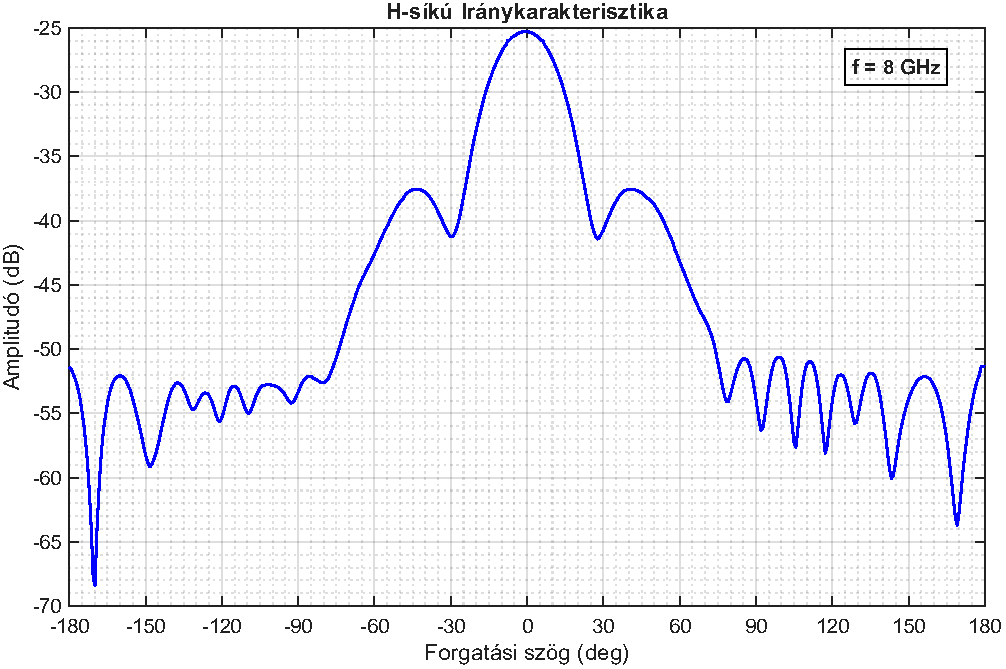
\includegraphics[width=\textwidth]{gen_abrak/8_GHz_H-H_Plot.pdf}
         
     \end{subfigure}
     \hfill
     \begin{subfigure}[b]{0.3\textwidth}
         \centering
         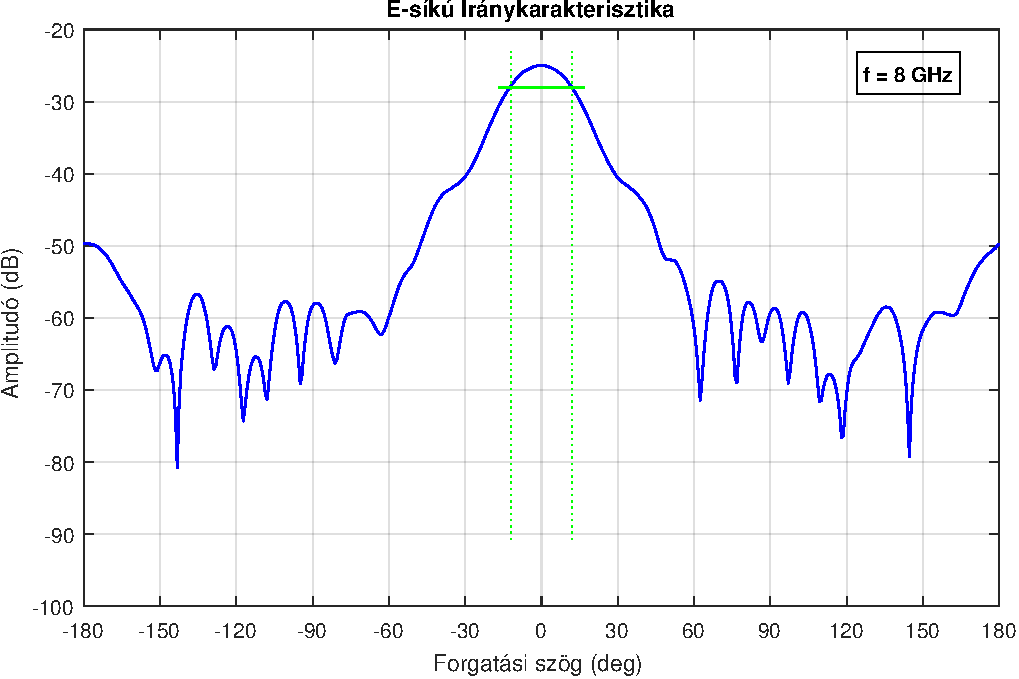
\includegraphics[width=\textwidth]{gen_abrak/8_GHz_V-V_Plot}
         
     \end{subfigure}
     \hfill
     \begin{subfigure}[b]{0.3\textwidth}
         \centering
         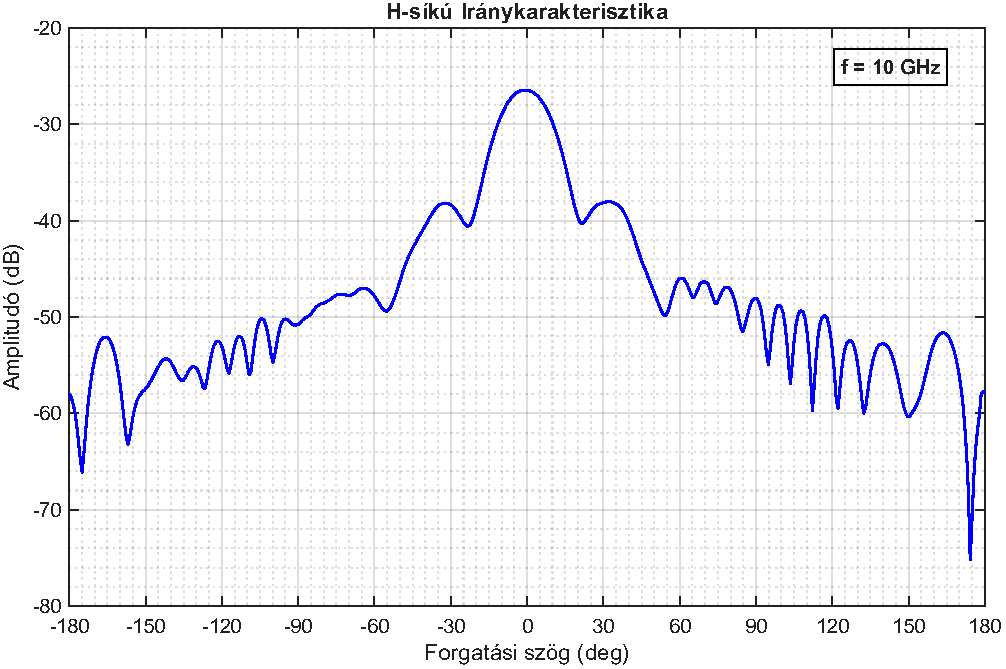
\includegraphics[width=\textwidth]{gen_abrak/10_GHz_H-H_Plot}
         
     \end{subfigure}

     \vspace{1em} % Adds vertical space between rows

     % --- Second Row ---
     \begin{subfigure}[b]{0.3\textwidth}
         \centering
         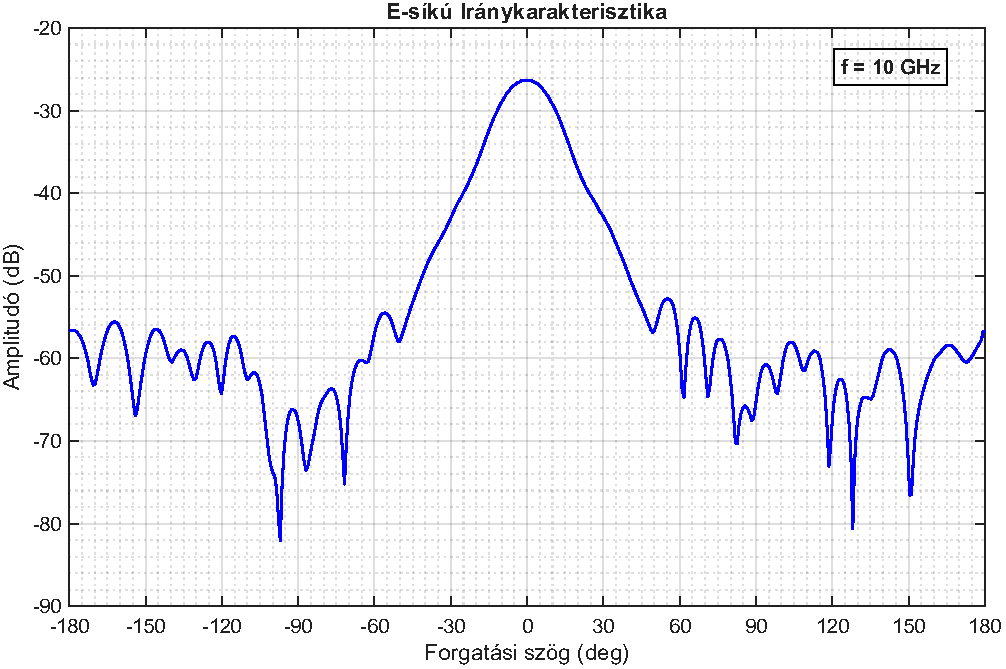
\includegraphics[width=\textwidth]{gen_abrak/10_GHz_V-V_Plot}
         
     \end{subfigure}
     \hfill
     \begin{subfigure}[b]{0.3\textwidth}
         \centering
         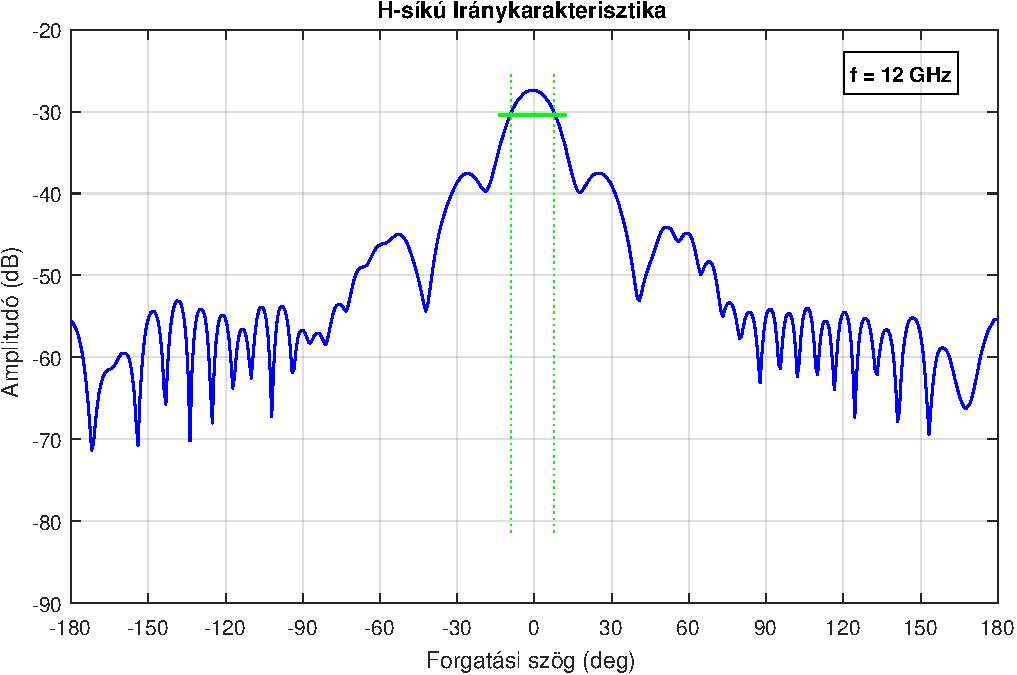
\includegraphics[width=\textwidth]{gen_abrak/12_GHz_H-H_Plot}
         
     \end{subfigure}
     \hfill
     \begin{subfigure}[b]{0.3\textwidth}
         \centering
         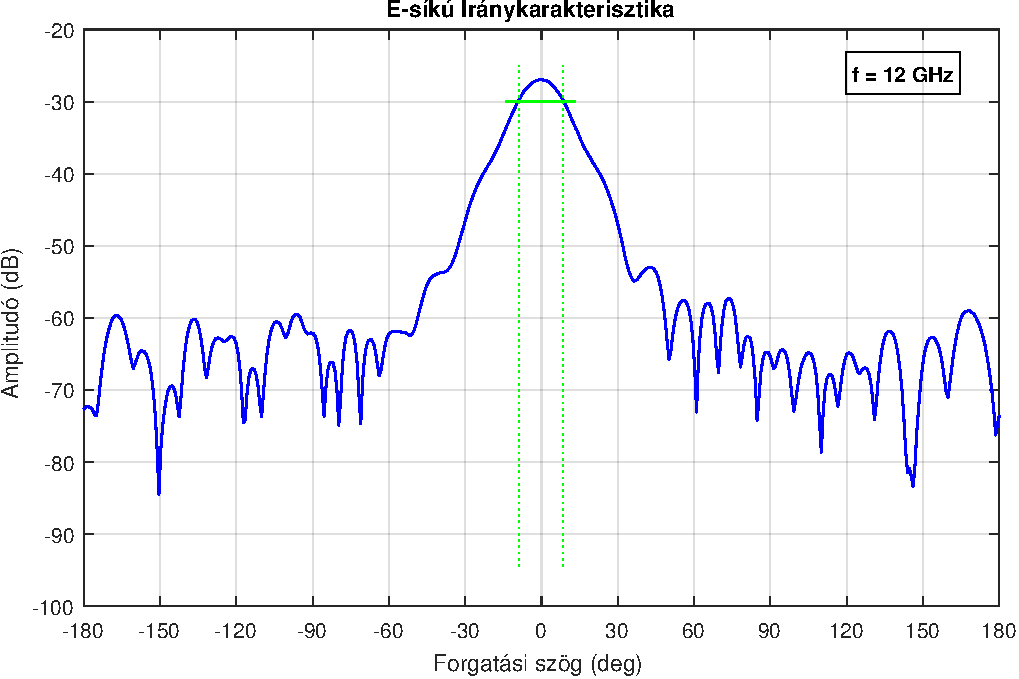
\includegraphics[width=\textwidth]{gen_abrak/12_GHz_V-V_Plot}
         
     \end{subfigure}
     
     \caption{Iránykarakterisztikák}
     \label{fig:irkar}
\end{figure}

\end{document}
\end{document}documentclass{article}
\usepackage{graphicx} % Required for inserting images
\usepackage[magyar]{babel}
\usepackage[T1]{fontenc}
\usepackage[utf8]{inputenc}
\usepackage{amsmath}
\usepackage{hyperref}
\usepackage{subcaption}
\title{
3.~Mérés - Antenna Iránykarakterisztika\\Mérési Beszámoló\vspace{1em}

\large Mérésvezető: dr. Lénárt Ferenc\\ B csoport}

\author{Bóta Barnabás \and Kovács Ágoston \and Valkai Máté}

\date{2026.03.04.}

\hyphenation{i-rány-ka-rak-te-risz-ti-ka}

\newcommand{\parrtp}{\left(r,\vartheta,\varphi\right)}
\newcommand{\partp}{\left(\vartheta,\varphi\right)}

\begin{document}

\maketitle
\tableofcontents{}
\section{A mérés célja, feladatok}
A mérés során gyakorlati tapasztalatokat szereztünk egy X-tölcsérantenna iránykarakterisztikájának meghatározásban. Több frekvencián is megvizsgáltuk az antenna viselkedését, valamint előállítottuk a tölcsérantenna azonos polarizációs, $E$- és $H$-síkú, valamint keresztpolarizációs amplitúdó iránydiagramjait. Végül pedig megmértük az antenna nyereségét kétantennás módszerrel.
\section{Elmélet, hasznos fogalmak}
\subsection{Az antennahatásfok irány- és polarizációfüggése}
Az antennára gondolhatunk úgy, mint egy transzformátorra egy hullámvezető és a szabad tér között. Mind a vevő- és szóróantenna a tér különböző irányaiba eltérő intenzitással sugároz, illetve eltérő érzékenységet mutat, azaz az antennára térbeli szűrőként tekinthetünk. 

A térbeli szűrő jelleg az  \textbf{iránykarakterisztikával} jellemezhető, amely gömbi vagy hengerkoordináta rendszerben ábrázolva mutatja be az előállított térerősség nagyságát. Az \textbf{iránydiagram} ennek az iránykarakterisztikának tuladjonképpen egy adott tengely szerinti síkmetszete.

Továbbá, egy antenna maximális hatásfokkal csak egyetlen polarizáció kisugárzására, vagy
vételére alkalmas. Az ettől eltérő polarizációs szög függvényében a hatásfok csökken,
ortogonális polarizáció esetén teljes elnyomás érvényesül. Az antenna polarizációja szintén irányfüggő lehet, vagyis a polarizációs elnyomás is tekinthető egyfajta szűrésnek. A polarizációt a komplex
\begin{equation}
\mathbf{p}\partp=p_n\partp\cdot\mathbf{\hat e}_n+p_x\partp\cdot\mathbf{\hat e}_x
\label{eq:polar}
\end{equation}
polarizációs iránykarakterisztikával jellemezhetjük, ahol a használt koordináta-rendszer egységvektorai rendre a maximális hatásfokhoz tartozó névleges és az arra merőleges keresztpolarizációs egységvektorok.
Ennek felhasználásával a távoltér egy meghatározott pontjában előállított térerősséget kifejezhetjük az adott távolságra érvényes $\mathbf{E}_\text{max}\parrtp$ térerősségmaximum és az $F\partp$ amplitúdó iránykarakterisztika szorzatával:
\begin{equation}
\mathbf E\parrtp=\left|\mathbf{E}_\text{max}\parrtp \right|\cdot F\partp\cdot\mathbf{p}\partp.
\label{eq:field}
\end{equation}

A gyakorlatban a komplex vektor iránykarakterisztika nehéz kezelhetősége miatt a polarizációs komponensek szerinti két összetevővel szokás jellemezni az antennát, amiben megjelenik annak adott komponensre vonatkozó $\left|F\partp\right|$ amplitudó karakterisztikája és $\Phi\partp$ fáziskarakterisztikája. A keresztpolarizációs komponens leírásához ugyanakkor elegendő az $a_x$ keresztpolarizációs csillapítás  megadása. 
\begin{gather}
    F_n\partp=\frac{E_n\partp}{E_{n,\text{ max}}}=\left|F_n\partp\right|e^{\mathrm j\Phi_n\partp}\\
    a_x\partp\left[\mathrm{dB}\right]=20\log\frac{p_n\partp}{p_x\partp}
\end{gather}
%ide ábra?
\subsection{A mérés során felhasznált további összefüggések}
\begin{description}

    \item[Nyereség:] Megadja, hogy a vizsgált antenna a fő sugárzási irányában mennyivel nagyobb térerősséget hoz létre, mint egy izotróp\footnote{Idealizált, az antennát minden irányba azonos teljesítménnyel sugárzóként vagy azonos nyereséggel vevőként leíró modell.} antenna, azonos bemenő teljesítmény mellett: \[G=\frac{S_\text{max}}{S_0},\ \text{ahol}\ S_0=\frac{P_\text{be}}{4\pi\cdot r^2}.\]

    \item[Irányhatás:] Annak mérőszáma, hogy a vizsgált antenna a főirányában hányszoros teljesítménysűrűséget állít elő az ugyanakkora teljesítményt kisugárzó izotróp antennához képest: \[D=\frac{S_\text{max}}{S_0},\ \text{ahol}\ S_0=\frac{P_\text{kisugárzott}}{4\pi\cdot r^2}.\]

    \item[Minimális mérési távolság:] A távoltér biztosításának egy fontos feltétele a megfelelő $R_\text{min}$ mérési távolság beállítása. Ezzel elérjük, hogy az adóantennából kiinduló gömbhullámok a mérőantennánál már elegendően kis fázishibával gömbhullámoknak tekinthetők. $\frac\lambda{16}$-nál kisebb fázishibát megengedve: \[R_\text{min}=\frac{2D^2}\lambda,\]
    ahol \begin{itemize}
        \item $D$ az antenna terjedési irányra merőleges mérete,
        \item $\lambda$ pedig a szabadtéri hullámhossz.
    \end{itemize}
\end{description}
\section{A mérés menete}
\subsection{Helyszín}
A távoltéri iránykarakterisztika méréséhez szükséges akadálymentes szabad teret nehezen
találunk, azt általában ki kell alakítani. A mi esetünkben beltéren került sor a mérésre, amely esetben reflexiómentesítő anyagokat használnak a mérőtérben lévő objektumokról reflektálódó elektromágneses sugárzás
intenzitásának csökkentésére.

A reflexiómentesítő anyagok működése azon alapul, hogy belépő felületükön közegjellemzőik kevéssé térnek el a szabadtéritől, belsejükben viszont jelentősen csillapodik az áthaladó elektromágneses hullám. Ennek hatására a belépő felületről reflektálódó teljesítmény szintje alacsony lesz, miközben az elfedett zavaró objektum hatása is jelentősen csökken.

A zavaró reflexiókat természetesen nem tudjuk zérusra, csak egy alkalmas szint alá csökkenteni. A mérőtér azon részét, ahol ez teljesül csendes zónának nevezik.

\section{Mérési eredmények}
\begin{figure}[hbtp]
     \centering
     % --- First Row ---
     \begin{subfigure}[b]{0.5\textwidth}
         \centering
         
\includegraphics[width=\textwidth]{8_GHz_H-H_Plot.pdf}
     \end{subfigure}
     \hfill
     \begin{subfigure}[b]{0.5\textwidth}
         \centering
         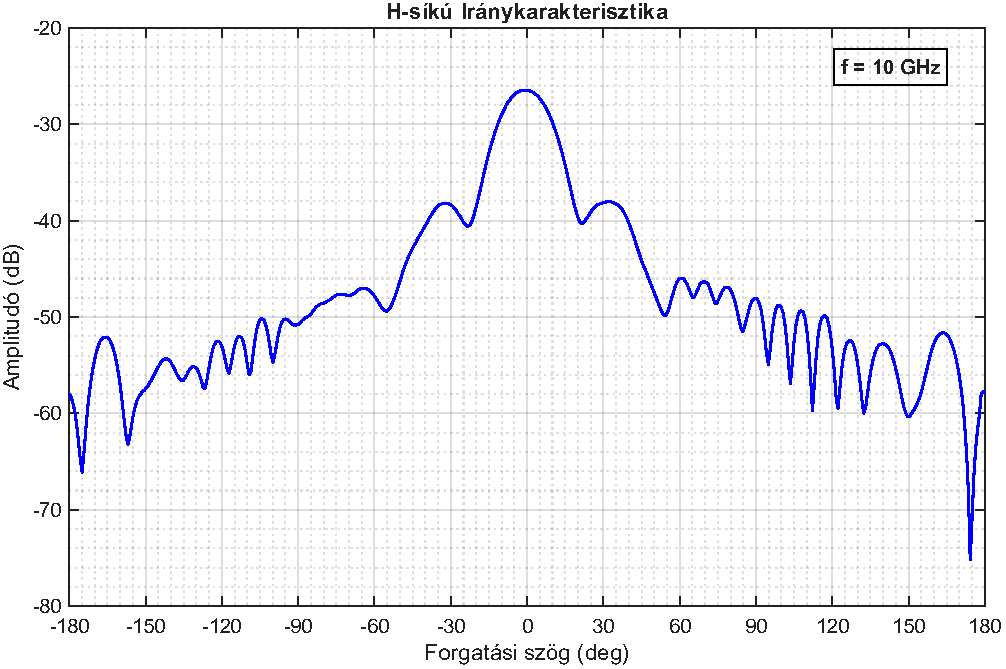
\includegraphics[width=\textwidth]{gen_abrak/10_GHz_H-H_Plot}
     \end{subfigure}
     % --- Second Row ---
     \begin{subfigure}[b]{0.5\linewidth}
         \centering
         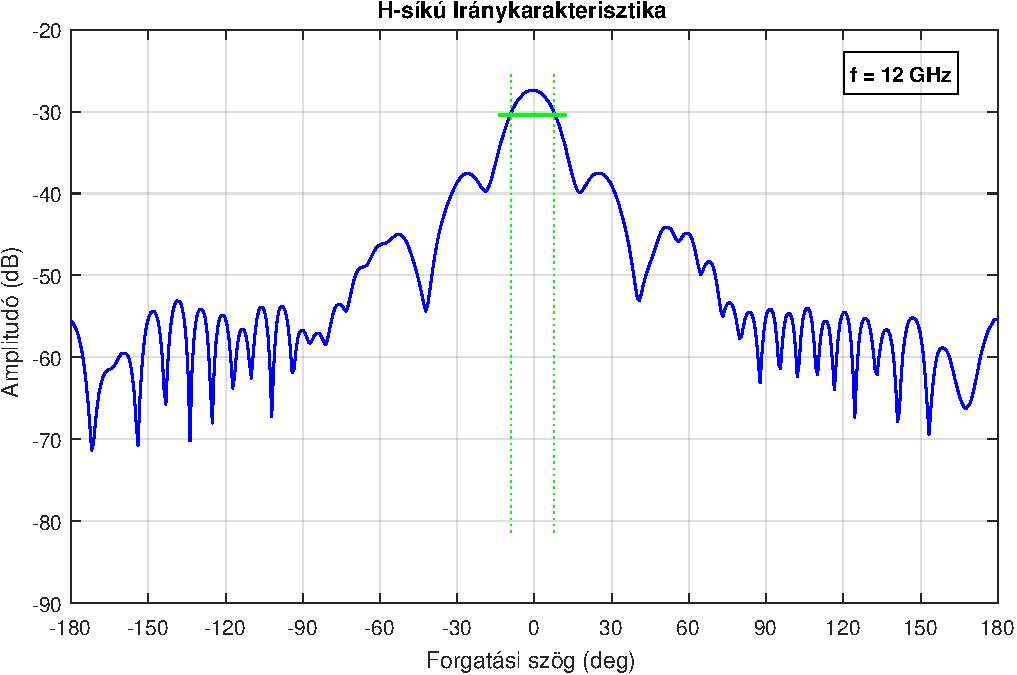
\includegraphics[width=\linewidth]{gen_abrak/12_GHz_H-H_Plot}
     \end{subfigure}
     \caption{Iránykarakterisztikák}
     \label{fig:irkarH}
\end{figure}
\begin{figure}[hbtp]
     \centering
     \begin{subfigure}[b]{0.5\textwidth}
         \centering
         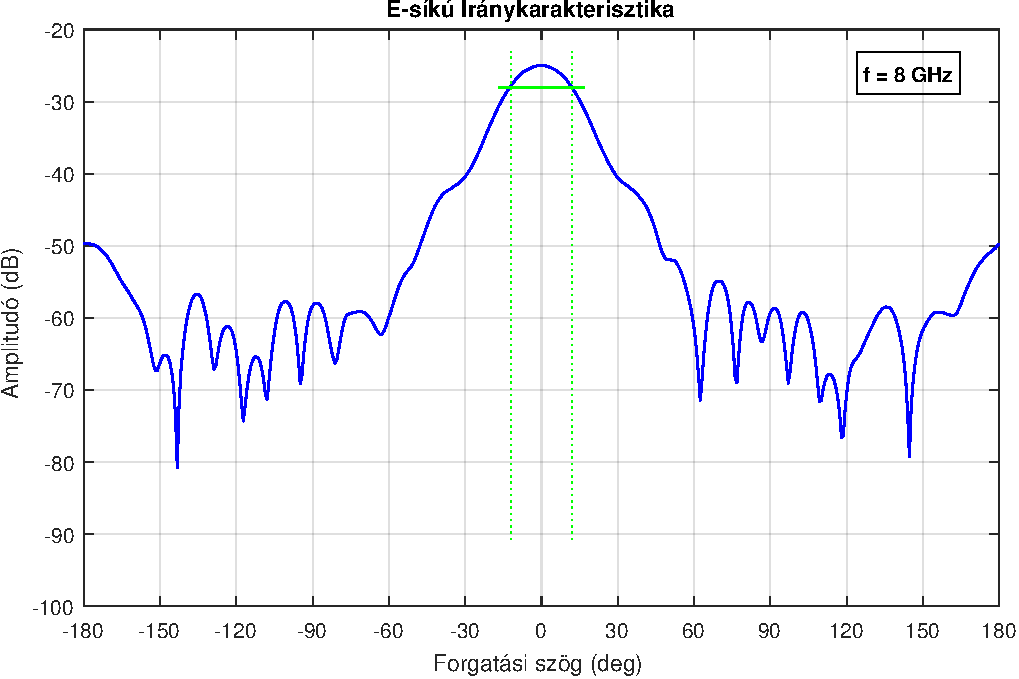
\includegraphics[width=\textwidth]{gen_abrak/8_GHz_V-V_Plot}
     \end{subfigure}
     \hfill
     % --- Second Row ---
     \begin{subfigure}[b]{0.5\linewidth}
         \centering
         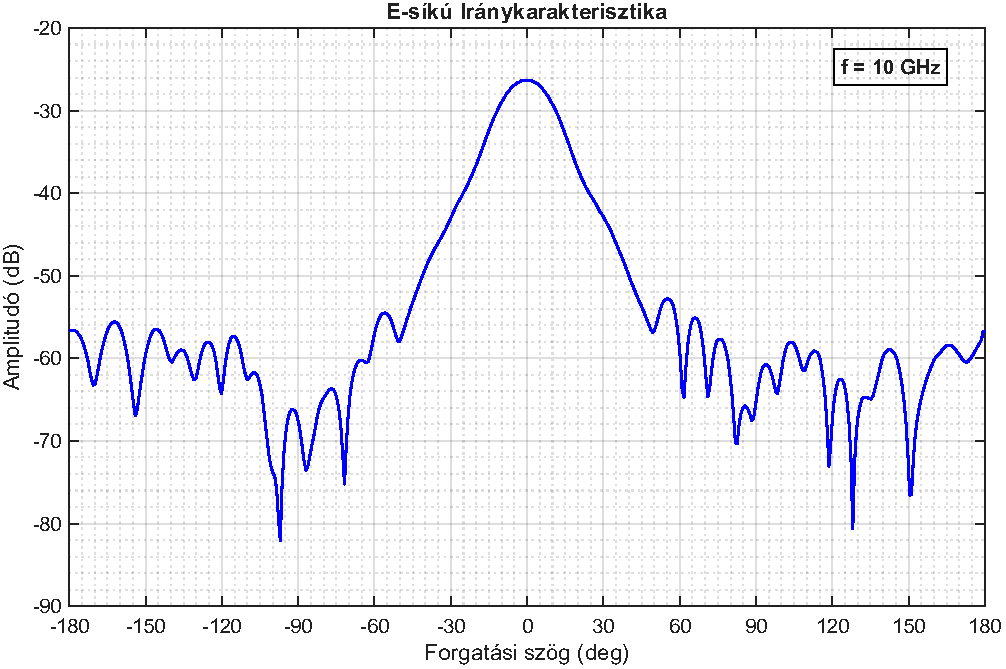
\includegraphics[width=\textwidth]{gen_abrak/10_GHz_V-V_Plot}
     \end{subfigure}
     \hfill
     \end{subfigure}
     \hfill
     \begin{subfigure}[b]{0.5\linewidth}
         \centering
		 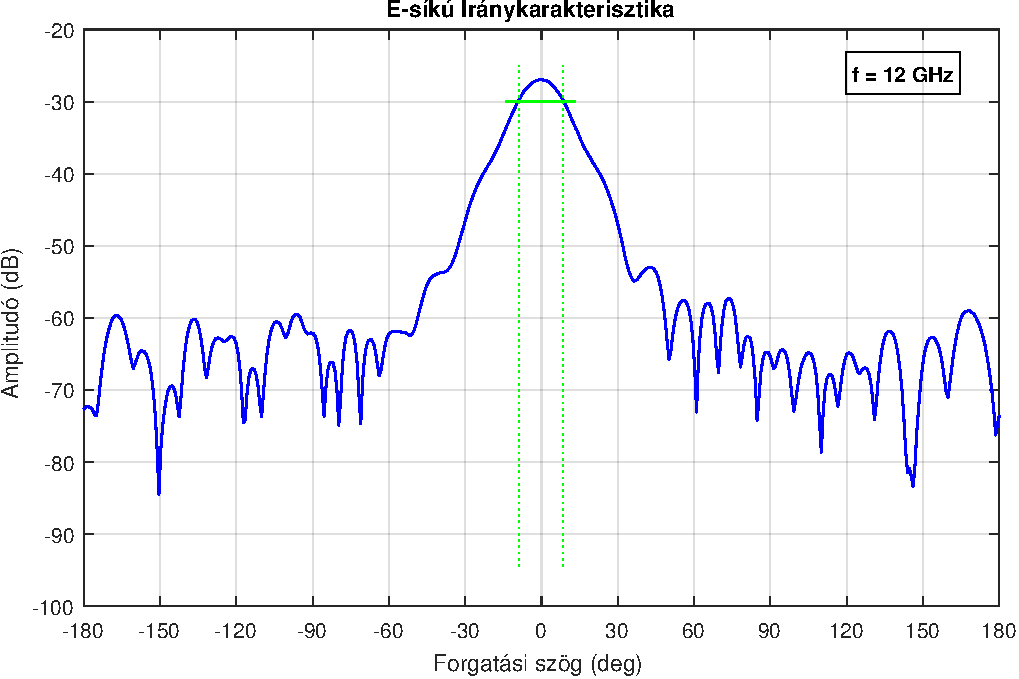
\includegraphics[width=\linewidth]{gen_abrak/12_GHz_V-V_Plot}
     \end{subfigure}
     \caption{Iránykarakterisztikák}
     \label{fig:irkarV}
\end{figure}
\end{document}
\end{document}
